%DGraph_counter_example_original



\documentclass{standalone}
% newcommands.tex

\newcommand{\enq}{\texttt{enq}}
\newcommand{\deq}{\texttt{deq}}
\newcommand{\pput}{\texttt{PUT}}
\newcommand{\get}{\texttt{GET}}
\newcommand{\vs}{\texttt{vis}}
\newcommand{\so}{\texttt{so}}
\newcommand{\arb}{\texttt{ar}}
\newcommand{\rf}{\texttt{rf}}

% example
\newcommand{\po}[2]{\draw [->, thick] (#1) to node[above] {\Large{\so}} (#2);}
\newcommand{\pva}[2]{\draw [->, thick] (#1) to node[above] {$\Large{\so},\Large{\vs},\Large{\arb}$} (#2);}
\newcommand{\pbva}[2]{\draw [->, thick] (#1) to node[above] {$\Large{\so}$} node[below] {$\Large{\vs},\Large{\arb}$} (#2);}
\newcommand{\pv}[2]{\draw [->, thick] (#1) to node[above] {\Large{\so}} node[below] {\Large{\vs}} (#2);}
\newcommand{\evis}[2]{\draw [->, thick] (#1) to node[above, sloped, near end] {\Large{\vs}} (#2);}
\newcommand{\mvis}[2]{\draw [->, thick] (#1) to node[above, sloped] {\Large{\vs}} (#2);}
\newcommand{\ar}[2]{\draw [->, thick, allow upside down] (#1) to node[above, sloped] {\Large{\arb}} (#2);}
\newcommand{\va}[2]{\draw [->, thick, allow upside down] (#1) to node[above, sloped] {$\Large{\vs},\Large{\arb}$} (#2);}
\newcommand{\vab}[2]{\draw [->, thick, allow upside down] (#1) to node[below, sloped, near end] {$\Large{\vs},\Large{\arb}$} (#2);}
\newcommand{\vae}[2]{\draw [->, thick, allow upside down] (#1) to node[above, sloped, near end] {$\Large{\vs},\Large{\arb}$} (#2);}
\newcommand{\vas}[2]{\draw [->, thick, allow upside down] (#1) to node[sloped, near start, above] {$\Large{\vs},\Large{\arb}$} (#2);}

% serialization
\newcommand{\scc}[2]{\draw [->, very thick] (#1) to (#2);}
\newcommand{\rva}[2]{\draw [->, thick, allow upside down] (#1) to node[above, sloped] {$\Large{\rf},\Large{\vs},\Large{\arb}$} (#2);}
\newcommand{\rvb}[2]{\draw [->, thick, allow upside down] (#1) to node[below, sloped] {$\Large{\rf},\Large{\vs},\Large{\arb}$} (#2);}


\usepackage{tikz}
\usetikzlibrary{shapes, positioning, arrows.meta, decorations.pathmorphing}

\begin{document}

    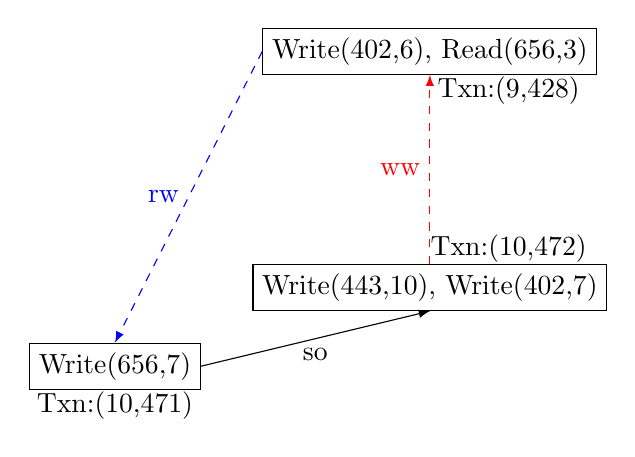
\begin{tikzpicture}[model/.style = {draw, minimum size = 15pt},  node distance = 0.5cm and 1.5cm]
        \node[model] (10472) at (0,0) {Write(443,10), Write(402,7)};
        \node (textof10472) at (1,0.5) {Txn:(10,472)};
        \node[model] (9428) at (0,3) {Write(402,6), Read(656,3)};
        \node (textof9428) at (1,2.5) {Txn:(9,428)};
        \node[model] (10471) at (-4,-1) {Write(656,7)};
        \node (textof10471) at (-4,-1.5) {Txn:(10,471)};
        \path[dashed, -latex, color=red] (10472.north) edge node[left] {ww} (9428.south); 
        \path[dashed, -latex, color=blue] (9428.west) edge node[left] {rw} (10471.north); 
        \path[-latex] (10471.east) edge node[below] {so} (10472.south); 
    \end{tikzpicture}

\end{document}